\xchapter{Desenvolvimento}{}

\section{Abordagem Geral}
Este trabalho adota uma abordagem de natureza aplicada e qualitativa, fundamentada em um experimento controlado com artefatos de um software real. O objetivo central consiste em investigar a eficácia de Modelos de Linguagem de Larga Escala  na verificação automatizada da conformidade entre requisitos, expressos em linguagem natural, e sua respectiva implementação no código-fonte. A metodologia proposta segue um fluxo estruturado que compreende a extração de arquivos de um repositório Git, a construção e o refinamento de prompts e, por conseguinte, a aplicação destes a diferentes modelos de linguagem por meio da ferramenta Gemini CLI e do GitHub Copilot integrado ao Visual Studio Code. As atividades foram conduzidas em um projeto concreto — o sistema “Nivelamento Online”, desenvolvido pela empresa Exatamente Soluções Educacionais, o que confere realismo e aplicabilidade prática à análise. Nesse contexto, busca-se avaliar a precisão das inferências geradas pelos modelos, os efeitos da engenharia de prompt e o impacto de distintas arquiteturas e configurações sobre a qualidade da verificação.

\section{Caracterização do Sistema sob Estudo}

O \textit{Nivelamento Online} (NiO) é uma plataforma educacional gamificada desenvolvida para apoiar o reforço de conteúdos escolares por meio de quizzes e atividades interativas. O sistema oferece modos de uso individual e coletivo, com funcionalidades voltadas tanto ao aluno quanto ao professor, incluindo a criação de perguntas, acompanhamento de desempenho e recursos de motivação baseados em mecânicas de jogo. 

Sua implementação adota a estrutura de múltiplos projetos, sendo os módulos de front-end e back-end os princiapis, além desses o repositório inclui outros componentes auxiliares relacionados à operação da plataforma. O front-end é construído como uma aplicação de página única (SPA) utilizando o framework Vue.js, sendo responsável pela interface e experiência do usuário. O back-end principal, por sua vez, é desenvolvido em Java com Spring Boot sendo dividido em multi módulos. Essa estrutura modular e multifacetada confere ao sistema uma complexidade significativa, especialmente no que diz respeito à rastreabilidade entre requisitos e implementações.

\section{Metodologia}

O percurso metodológico deste trabalho foi fundamentado em um processo iterativo, estruturado em seis etapas principais. Cada etapa representa uma fase distinta do experimento de verificação automatizada da conformidade entre requisitos e código-fonte, conforme descrito a seguir. 

\begin{enumerate}
    \item \textbf{Coleta de Artefatos:} A fase inicial consistiu na extração dos artefatos do sistema “Nivelamento Online”, diretamente de seu repositório Git. Foram coletados tanto os documentos de requisitos quanto os arquivos de código-fonte que serviram de base para o experimento. 
    \item \textbf{Formulação Inicial dos Prompts:} Com base nos requisitos, elaboraram-se prompts iniciais em linguagem natural, cujo propósito era instruir os modelos de linguagem a verificar a implementação de cada requisito. Tais prompts foram projetados para que os modelos classificassem os requisitos em categorias predefinidas (\textit{Implemented}, \textit{Partially}, \textit{Missing} ou \textit{Unknown}) e justificassem suas conclusões. 
    \item \textbf{Execução Inicial com LLMs:} Subsequentemente, os prompts foram submetidos a diferentes modelos de linguagem por meio da ferramenta Gemini CLI e, paralelamente, via GitHub Copilot no Visual Studio Code. Essa execução inicial estabeleceu uma linha de base para a avaliação de desempenho. 
    \item \textbf{Refinamento com Engenharia de Prompt:} A análise dos resultados preliminares permitiu identificar falhas interpretativas e limitações. Diante disso, os prompts foram aprimorados com o uso de técnicas de engenharia de prompt, como \textit{few-shot prompting} (inserção de exemplos) e \textit{chain-of-thought prompting} (estímulo ao raciocínio em cadeia), objetivando maior robustez e rastreabilidade semântica. 
    \item \textbf{Reexecução com Prompts Refinados:} Os prompts otimizados foram então reaplicados aos mesmos modelos e ambientes. Essa etapa foi crucial para comparar diretamente o desempenho antes e depois do refinamento, permitindo, assim, mensurar o impacto das técnicas de engenharia de prompt. 
    \item \textbf{Coleta e Análise dos Resultados:} Por fim, todas as respostas geradas foram sistematicamente registradas, categorizadas e avaliadas. As análises abrangeram a validação das respostas e a medição da acurácia, taxa de omissão, precisão, \textit{recall} e \textit{F1-score}. Essas métricas foram utilizadas por serem amplamente reconhecidas na literatura como indicadores robustos para avaliar classificadores, permitindo mensurar não apenas a proporção de acertos, mas também a capacidade dos modelos em evitar falsas classificações e identificar corretamente os requisitos relevantes. Os dados foram consolidados em tabelas de desempenho para viabilizar uma interpretação quantitativa e qualitativa do comportamento dos modelos.
\end{enumerate}

% A utilização de métricas quantitativas revelou-se essencial para avaliar objetivamente o desempenho dos modelos aplicados à verificação automatizada de conformidade entre requisitos e código-fonte. Neste experimento, duas métricas foram particularmente relevantes: a acurácia e a taxa de omissão. A acurácia permite mensurar a proporção de classificações corretas, isto é, em que o modelo atribuiu o rótulo adequado ao requisito analisado, em relação ao total de casos avaliados. Trata-se de uma métrica abrangente, que fornece uma visão geral da performance do modelo, considerando tanto acertos em requisitos implementados quanto corretamente identificados como ausentes. 

% Já a taxa de omissão foi empregada para capturar um tipo específico de falha: situações em que o modelo não forneceu nenhuma resposta em requisitos cuja implementação estava de fato presente no código. Em contextos de engenharia de software, esse tipo de erro pode comprometer significativamente a rastreabilidade e a confiabilidade do processo de auditoria, ao deixar requisitos efetivamente atendidos sem o devido reconhecimento. Assim, a análise combinada da acurácia e da taxa de omissão fornece uma visão crítica sobre a capacidade do modelo de não apenas acertar, mas também de evitar silêncios injustificados diante de evidências válidas.

\subsection{Seleção dos casos de teste.}
Para condução do experimento, foram selecionados dois documentos de caso de teste provenientes de módulos distintos do sistema. O primeiro corresponde à funcionalidade de geração automatizada de questões com apoio de Inteligência Artificial, a qual envolve tanto componentes de \textit{back-end} quanto de \textit{front-end}, sendo referenciada nos testes como módulo \textbf{IA}. Essa funcionalidade permite que o usuário submeta um documento contendo conteúdo pedagógico ou uma descrição textual, com o objetivo de que a IA extraia automaticamente questões coerentes com o material fornecido e as insira diretamente na base de dados do sistema. Trata-se, portanto, de uma funcionalidade que combina processamento textual, análise semântica e integração com o fluxo de criação de atividades dentro da plataforma.

O segundo módulo selecionado, identificado como \textbf{REL}, refere-se à geração de relatórios de desempenho de alunos ou jogadores. Embora o sistema já ofereça visualizações gráficas e estatísticas no ambiente online, essa funcionalidade foi desenvolvida para permitir que professores ou organizadores exportem os dados consolidados em um arquivo no formato \texttt{.xlsx}, compatível com softwares de planilha. Essa opção proporciona uma visão abrangente, offline e reutilizável dos dados, o que é especialmente útil para análise detalhada, arquivamento ou compartilhamento externo dos resultados. A implementação do módulo REL encontra-se majoritariamente no \textit{back-end}, concentrando-se em operações de consulta, agregação e formatação dos dados educacionais.

Esses dois módulos foram escolhidos por representarem tipos distintos de desafio técnico, um com foco em integração com IA e requisição assíncrona, e outro com lógica de negócio intensiva no servidor e alto valor analítico. Os documentos de teste correspondentes serviram como base para a extração dos requisitos e cenários avaliados pelas IAs, e seus identificadores foram mantidos nos resultados (\texttt{IA-RF01}, \texttt{REL-RF02}, etc.) para permitir o rastreio da origem durante a análise.

\section{Visão Arquitetural da Solução}

Para contextualizar a solução proposta, foi utilizado o modelo C4, que permite representar a arquitetura de software em diferentes níveis de abstração. As Figuras~\ref{fig:c4_contexto} e~\ref{fig:c4_containers} apresentam, respectivamente, os diagramas de contexto e de containers, que, juntos, oferecem uma visão geral do fluxo operacional da solução e da organização de seus principais componentes.

\begin{figure}[H]
    \centering
    \begin{adjustbox}{width=0.9\textwidth,center}
        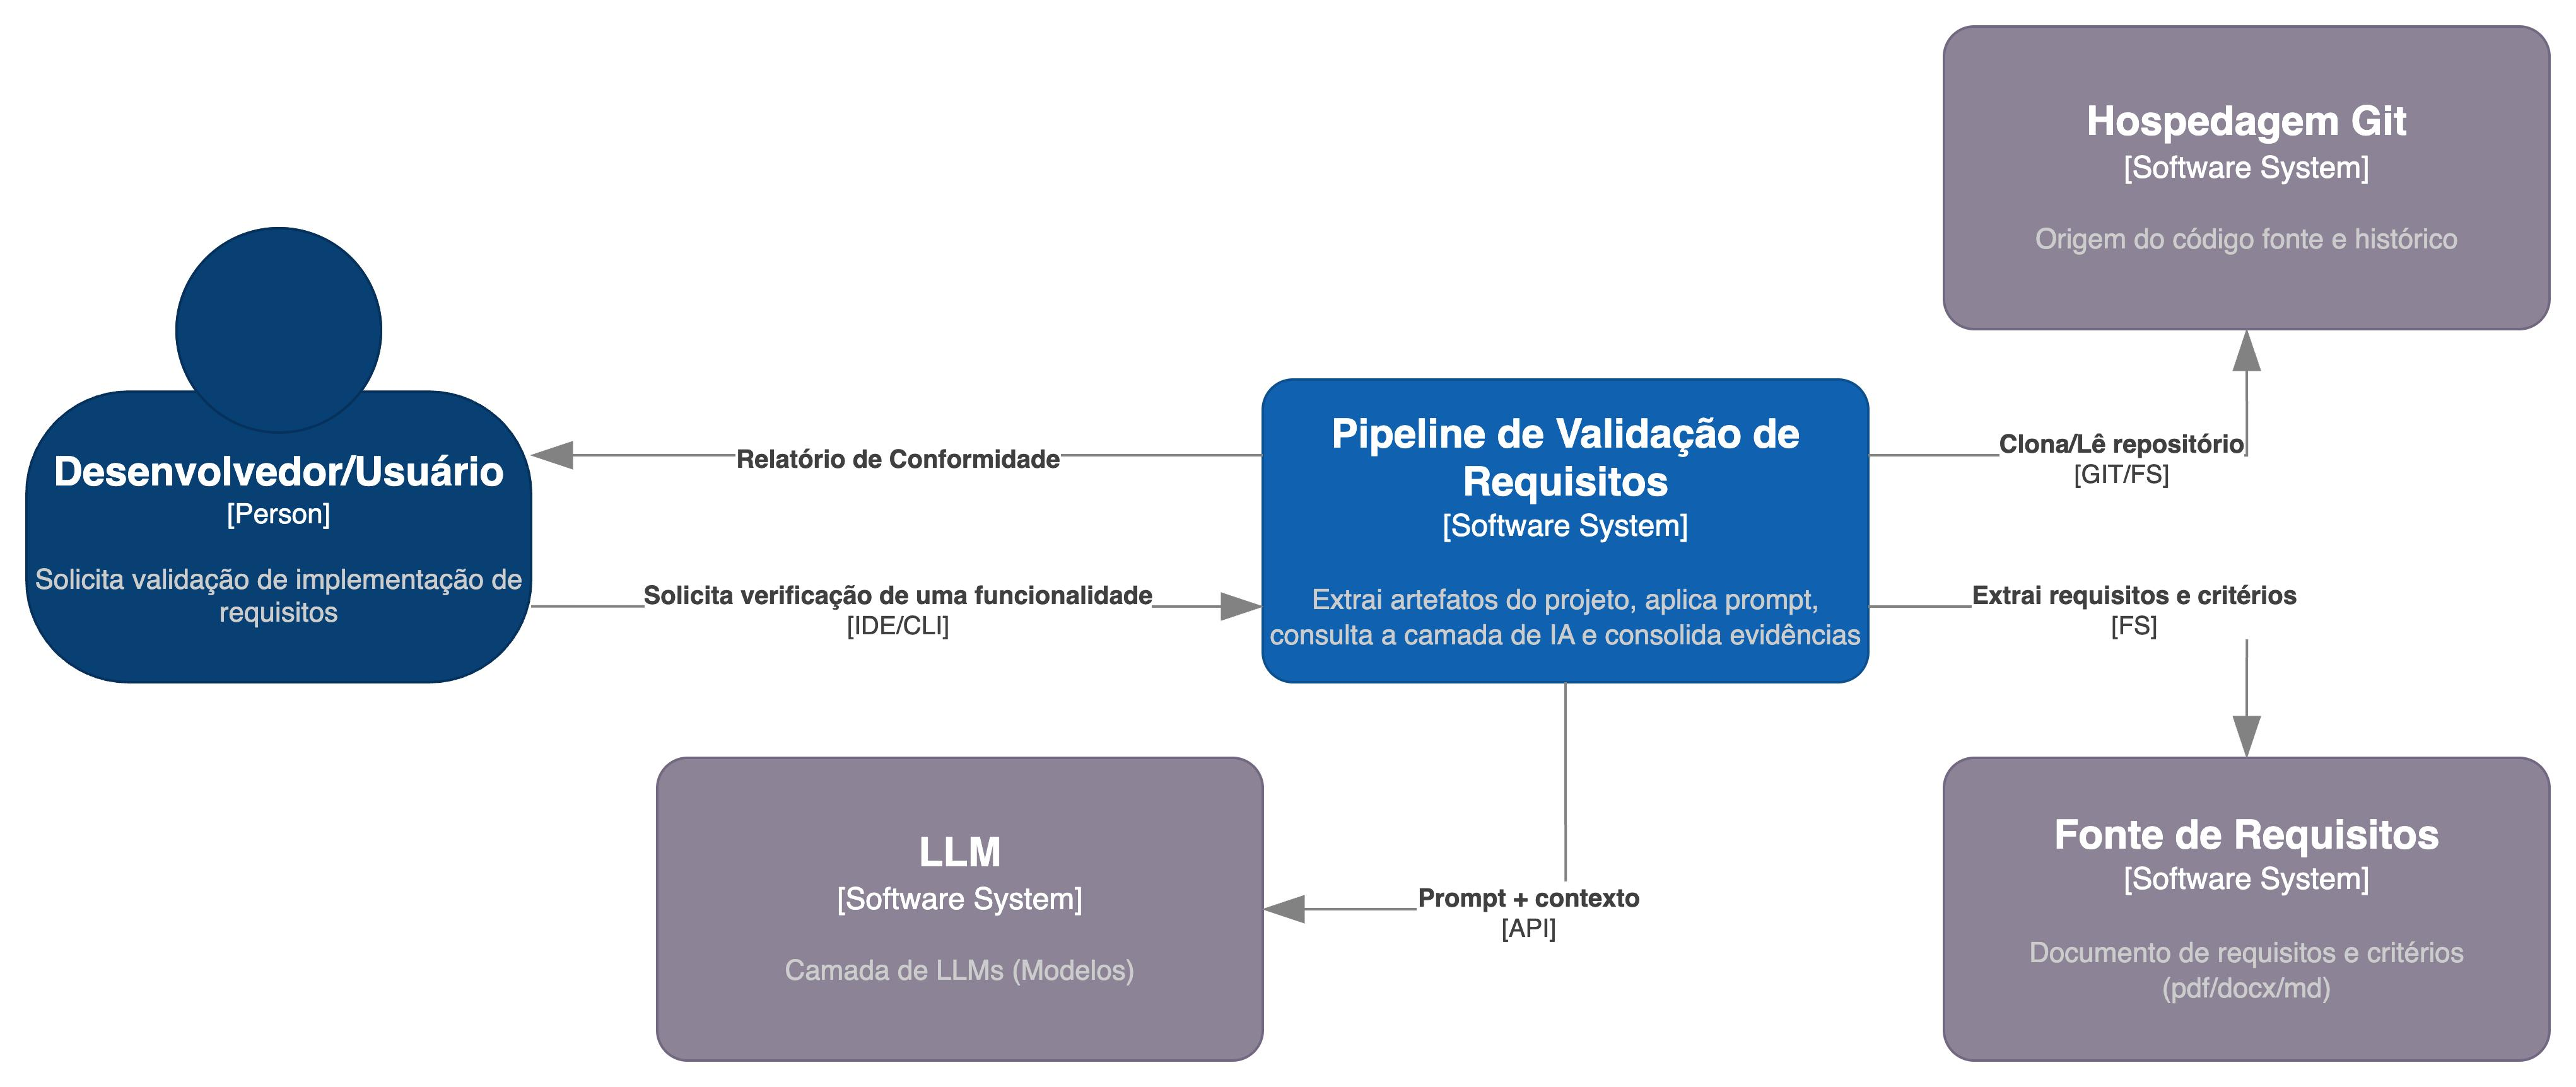
\includegraphics{imgs/c4_context.jpeg}
    \end{adjustbox}
    \caption{Diagrama de Contexto (Fonte: Própria)}
    \label{fig:c4_contexto}
\end{figure}

\begin{figure}[H]
    \centering
    \begin{adjustbox}{width=1.0\textwidth,center}
        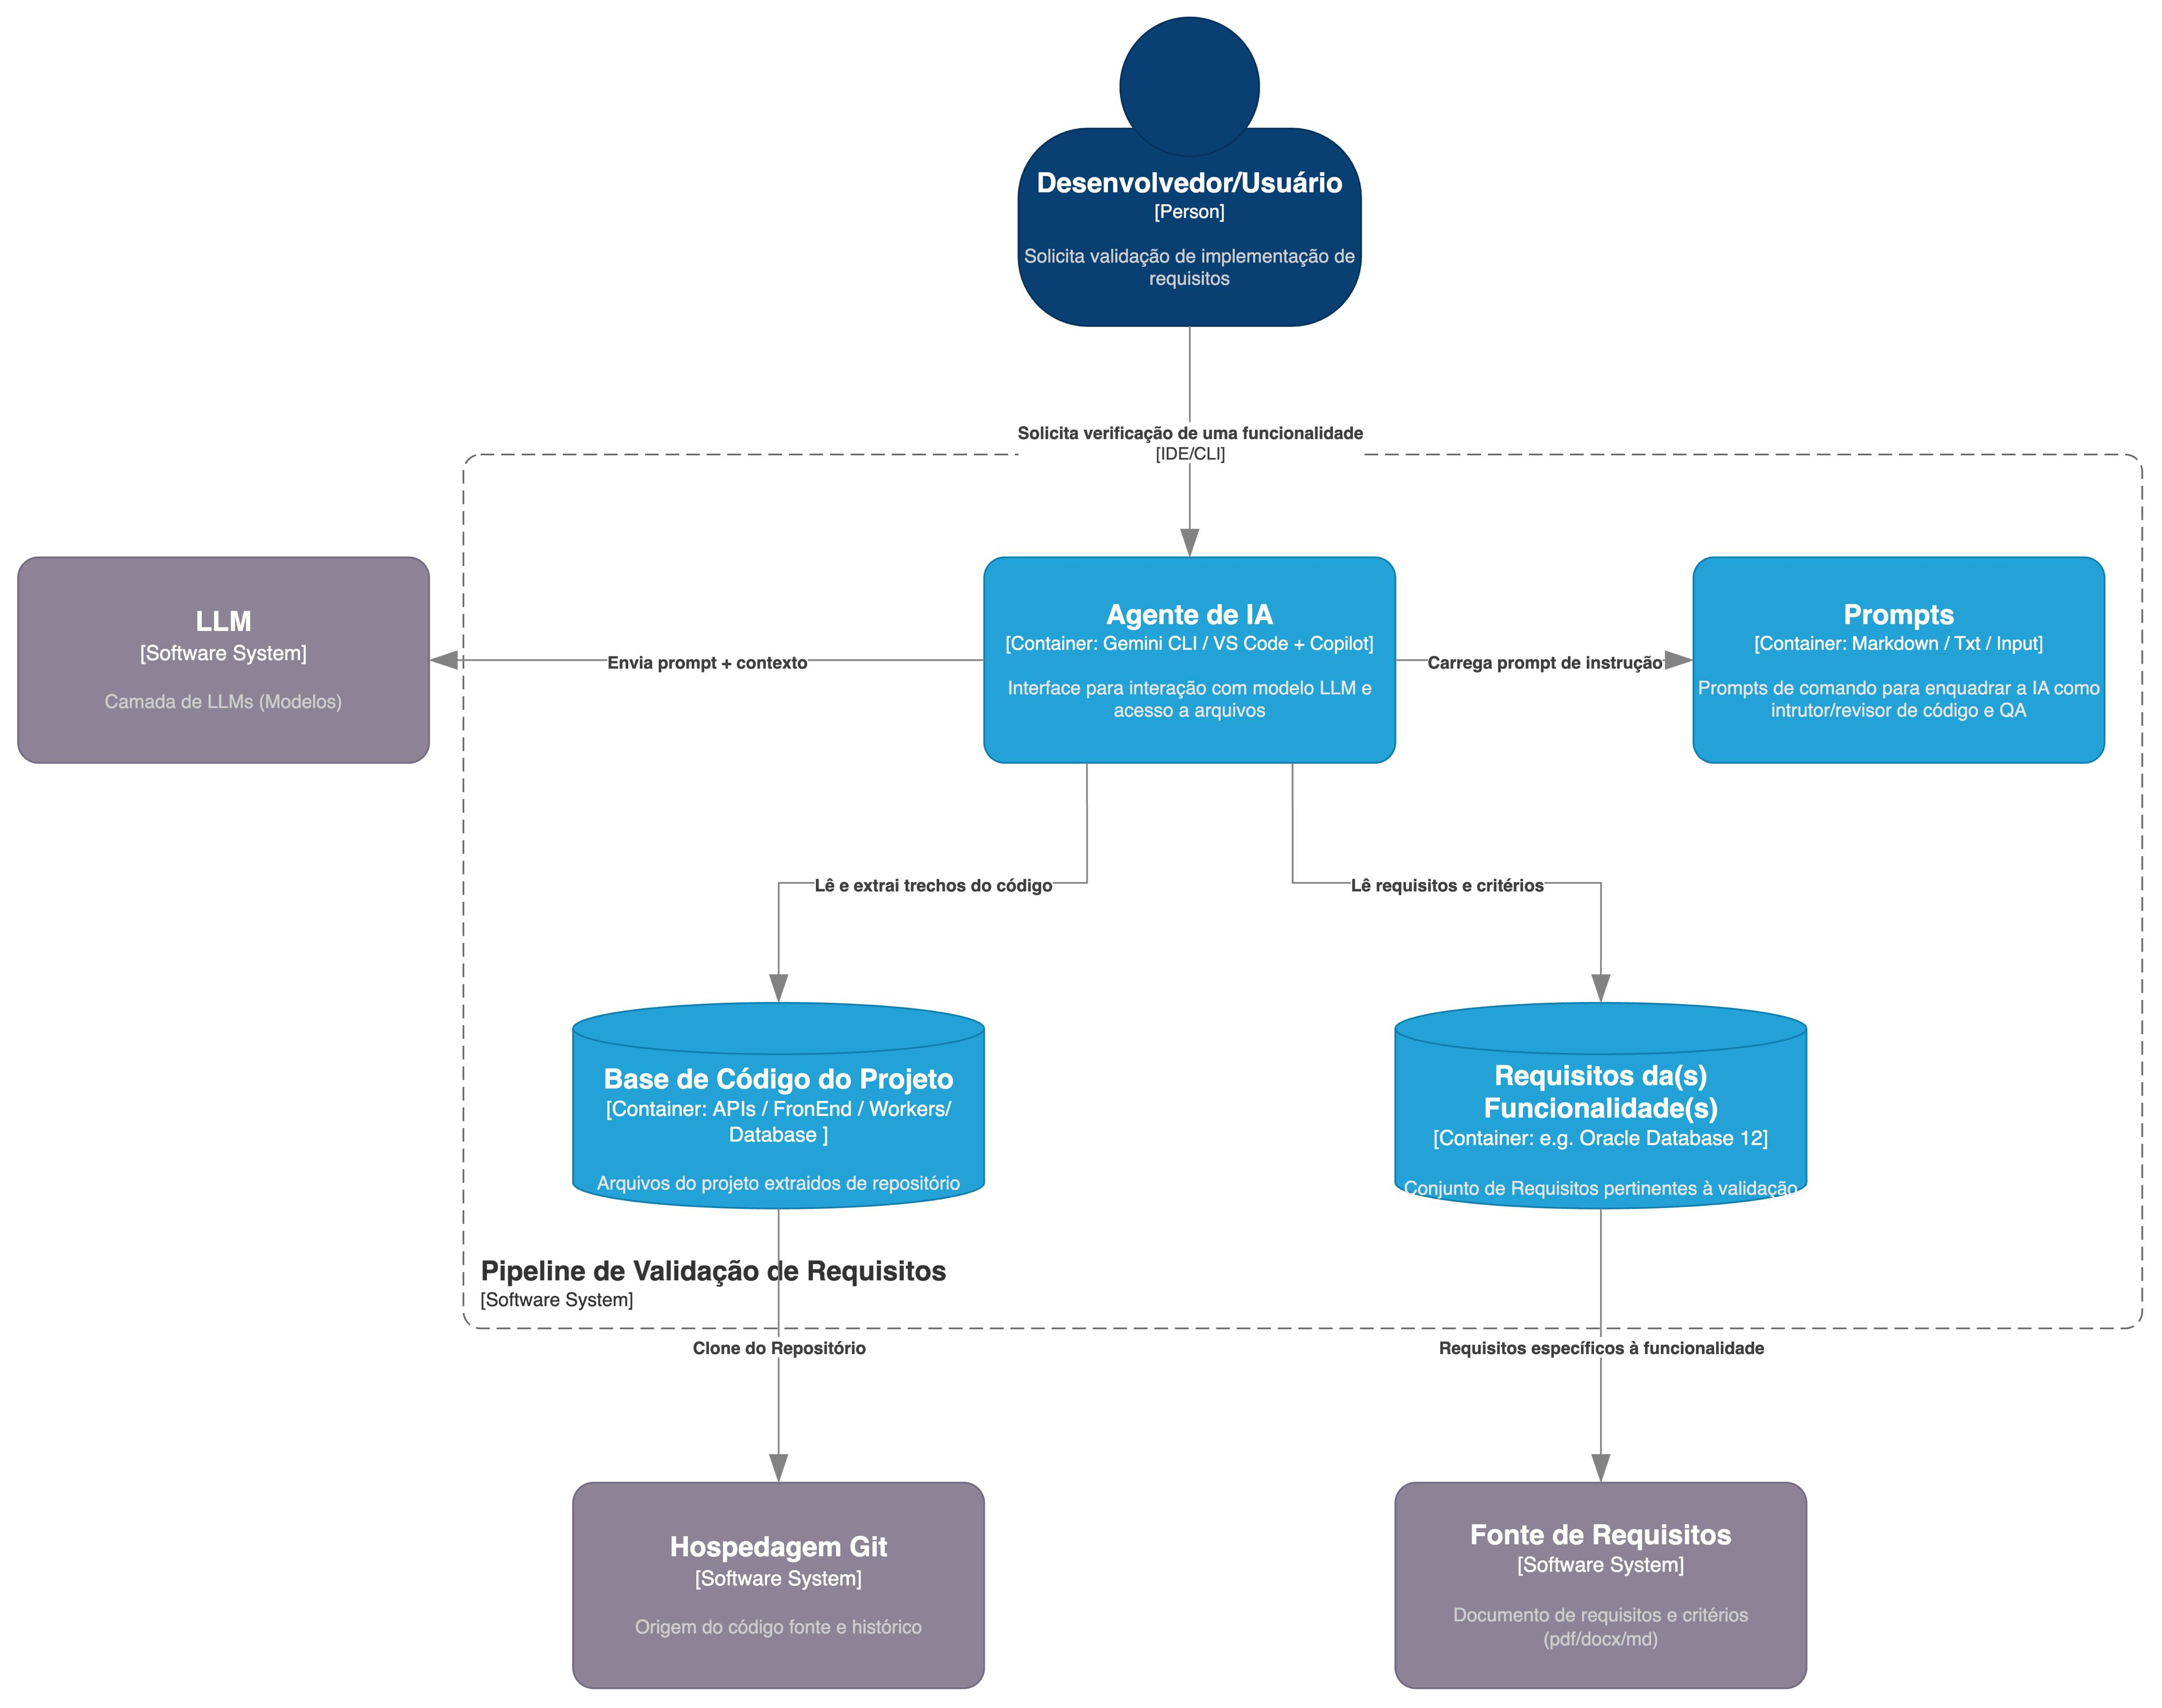
\includegraphics{imgs/c4_container.jpeg}
    \end{adjustbox}
    \caption{Diagrama de Containers (Fonte: Própria)}
    \label{fig:c4_containers}
\end{figure}

No diagrama de contexto (Figura~\ref{fig:c4_contexto}), observa-se que o processo tem início com a ação do usuário, que deseja validar se uma determinada funcionalidade foi implementada de acordo com os requisitos estabelecidos. Para isso, o usuário interage diretamente com o projeto local por meio de uma interface de linha de comando (CLI) ou uma interface gráfica no Ambiente de Desenvolvimento Integrado (IDE), ativando um conjunto estruturado de ações aqui denominado pipeline de validação de requisitos.

Essa pipeline consiste em operações realizadas localmente, como a leitura de arquivos do código-fonte e dos documentos de requisitos combinadas à construção de prompts, os quais serão utilizados como entrada para um modelo de linguagem (LLM), acessado remotamente via API. O modelo, por sua vez, retorna julgamentos ou explicações a respeito da conformidade entre os requisitos e os trechos de código analisados.

A Figura~\ref{fig:c4_containers} complementa essa visão ao detalhar os principais containers que participam do processo. O Agente de IA é representado como a interface de operação (CLI ou IDE), responsável por orquestrar o fluxo de validação, acessando diretamente os prompts, a base de código do projeto e os requisitos extraídos. Esse agente é responsável por preparar e enviar os dados ao modelo de linguagem, bem como interpretar as respostas e auxiliar na construção do relatório.

A base de código e os requisitos utilizados no processo são oriundos de repositórios hospedados externamente e previamente clonados ou armazenados na máquina local do usuário. Os prompts, por sua vez, são arquivos configuráveis (em Markdown ou texto estruturado) que orientam a atuação do agente como revisor, auditor ou verificador de conformidade.

Dessa forma, os dois diagramas apresentados fornecem uma visão consolidada do funcionamento da solução: um processo interativo, acionado localmente pelo usuário, que utiliza modelos de linguagem para auxiliar na análise semântica da aderência entre os requisitos documentados e o código-fonte implementado.


\subsection{Ferramentas e Modelos Utilizados}

O ambiente experimental foi configurado para permitir a comparação de desempenho entre diferentes modelos de linguagem de ponta, acessados por meio de duas interfaces principais. A seleção de múltiplos modelos visa observar variações na capacidade de interpretação e análise de código, conforme delineado nos objetivos específicos deste trabalho.

As ferramentas e os respectivos modelos utilizados foram:

\begin{itemize}
    \item Gemini CLI: Interface de linha de comando utilizada para interagir diretamente com o modelo Gemini 2.5 Pro.
    \item GitHub Copilot (integrado ao Visual Studio Code): A extensão foi configurada para alternar entre os seguintes modelos de apoio: Gemini 2.5 Pro, Claude Sonnet 4 e GPT 5.
\end{itemize}

Todos os testes foram executados mantendo os hiperparâmetros e configurações padrão dos modelos, a fim de garantir uma base de comparação consistente.


\section{Estruturação da Solução e Etapas do Experimento}
O sistema sob avaliação organiza, em um mesmo repositório, os módulos de \textit{front-end}, múltiplos serviços de \textit{back-end} e componentes adicionais (por exemplo, aplicativo móvel e serviços auxiliares). Para controlar efeitos de escopo durante a análise, foram definidos recortes explícitos da \textit{janela de contexto} disponibilizada ao agente. Nos cenários \textit{Front-end} e \textit{Back-end}, o modelo recebeu apenas os arquivos pertencentes às respectivas pastas. Consequentemente, quaisquer evidências existentes fora desse recorte ou cuja verificação exigisse informações não disponíveis no código visível deveriam ser classificadas como \textit{Unknown}. Por exemplo, ao avaliar um requisito de interface visual a partir do escopo do \textit{back-end}, o modelo não possui acesso à camada responsável, resultando em ausência de evidência observável. Da mesma forma, requisitos relacionados a tempo de resposta ou comportamento dinâmico da IA (como os presentes no módulo de geração automática de questões) não podem ser aferidos diretamente a partir do código-fonte, justificando também a classificação como \textit{Unknown} nesses casos.

No cenário de \textit{Repositório completo}, a IA teve acesso irrestrito a todos os diretórios do monorepositório, o que implica em um contexto mais amplo e heterogêneo para análise. Essa configuração exige que o modelo seja capaz de localizar, interpretar e correlacionar corretamente evidências distribuídas entre múltiplos serviços, camadas e tecnologias. Além da maior densidade informacional, o repositório apresenta estruturas semelhantes entre diferentes módulos, incluindo arquivos com nomes idênticos em contextos distintos, o que aumenta o risco de interpretações imprecisas. Tais características tornam o processo de rastreamento mais complexo, exigindo maior capacidade de filtragem semântica e distinção entre componentes funcionalmente próximos, mas logicamente independentes.

Os experimentos foram conduzidos em três contextos de análise:
\begin{enumerate}
    \item \textbf{Back-end}: análise restrita aos arquivos do servidor;
    \item \textbf{Front-end}: análise focada nos arquivos da interface do usuário;
    \item \textbf{Repositório completo}: análise abrangendo todos os módulos do sistema.
\end{enumerate}

Essa diversificação de cenários permitiu avaliar a capacidade do modelo de navegar pelos arquivos e identificar evidências em diferentes camadas arquiteturais. 

Após a primeira rodada, elaborou-se uma versão aprimorada do prompt, incorporando melhorias de engenharia de \textit{prompt} que visam reduzir ambiguidades e padronizar a tomada de decisão:

\begin{itemize}
    \item Objetivo geral mais abrangente, orientando a verificação de todo o conteúdo dos requisitos (critérios, restrições e regras de negócio), e não apenas do texto principal;
    \item Suporte explícito a múltiplos formatos de documentos de entrada (\texttt{.pdf}, \texttt{.md}, \texttt{.txt});
    \item Instruções de raciocínio estruturado (\textit{chain-of-thought}) para identificar o tipo de requisito, buscar evidências em múltiplos arquivos e fundamentar as inferências;
    \item Ênfase na navegação entre funções, serviços e classes, favorecendo uma inspeção mais profunda do código;
    \item Inclusão de uma tabela-guia com descrições e exemplos para cada rótulo de saída, padronizando as respostas;
    \item Exigência de justificativas objetivas, técnicas e não especulativas.
\end{itemize}

Com o \textit{prompt} revisado, repetiu-se a bateria de testes sobre os mesmos artefatos. Os resultados foram consolidados e comparados com os da rodada inicial, possibilitando mensurar o impacto da reescrita sobre acurácia, qualidade das explicações e taxa de omissões. Em seguida, os dados foram organizados para discutir o desempenho por modelo, \textit{prompt} e cenário avaliado.

\section{Experimentação e Evolução dos Prompts de Auditoria}

O processo de análise automatizada iniciou-se com a construção de um prompt-base, concebido para simular o comportamento de um auditor de conformidade de requisitos. 
\begin{minted}[fontsize=\small, breaklines=true, bgcolor=gray!5, linenos]{markdown}
# Prompt de Auditoria de Requisitos em Código

Você é um **auditor de conformidade de requisitos de software**.  
Sua tarefa é:

1. **Ler e interpretar requisitos de software** (funcionais e não funcionais), descritos em linguagem natural ou estruturada.  
2. **Verificar no projeto de software** (arquivos de código, configuração, testes, documentação técnica) se esses requisitos foram **Implementados**, **Parcialmente implementados**, **Não implementados (Missing)**, **Inconclusivos (Unknown)** ou **Contraditórios**.  
3. **Apresentar evidências concretas**, citando:
   - Caminho do arquivo (`path`)
   - Faixa de linhas (`start_line` – `end_line`)
   - Pequena justificativa de como o trecho atende ou não ao requisito.  

### Regras
- Não invente implementações. Se não houver evidência clara → responda `Unknown`.  
- Cite **apenas os trechos mínimos necessários** para justificar sua conclusão.  
- Quando aplicável, use múltiplas evidências (ex.: backend + frontend + testes).  
- Diferencie entre requisito funcional (o que o sistema deve fazer) e não funcional (como deve se comportar, p.ex. desempenho, segurança).  
- Use vocabulário objetivo e técnico, sem interpretações subjetivas.  

### Formato de Saída (JSON)

```json
[
  {
    "requirement_id": "REQ-001",
    "requirement_text": "Descrição do requisito em linguagem natural",
    "label": "Implemented | Partially | Missing | Unknown",  
    "evidence": [
      {
        "path": "src/.../Arquivo.java",
        "start_line": 120,
        "end_line": 140,
        "justification": "Este método valida assinatura PRO antes da geração."
      }
    ],
    "explanation": "Resumo curto do porquê desse rótulo.",
    "notes": "Incertezas, dependências ou sugestões de arquivos adicionais a revisar."
  }
]
\end{minted} 


Este prompt foi projetado para instruir o modelo de linguagem a executar uma tarefa complexa: analisar requisitos em linguagem natural e verificar sua implementação em artefatos como código-fonte, arquivos de configuração, testes e documentação técnica. O escopo do prompt inicial especificava um conjunto de categorias de classificação — \textit{Implemented}, \textit{Partially Implemented}, \textit{Missing} e \textit{Unknown}, além de requisitar evidências concretas para cada decisão, como o caminho do arquivo, a faixa de linhas e uma justificativa técnica. Além disso, as instruções determinavam que, na ausência de evidências claras, o requisito deveria ser classificado como \textit{Unknown} para evitar inferências subjetivas. 


\begin{figure}[H]
    \centering
    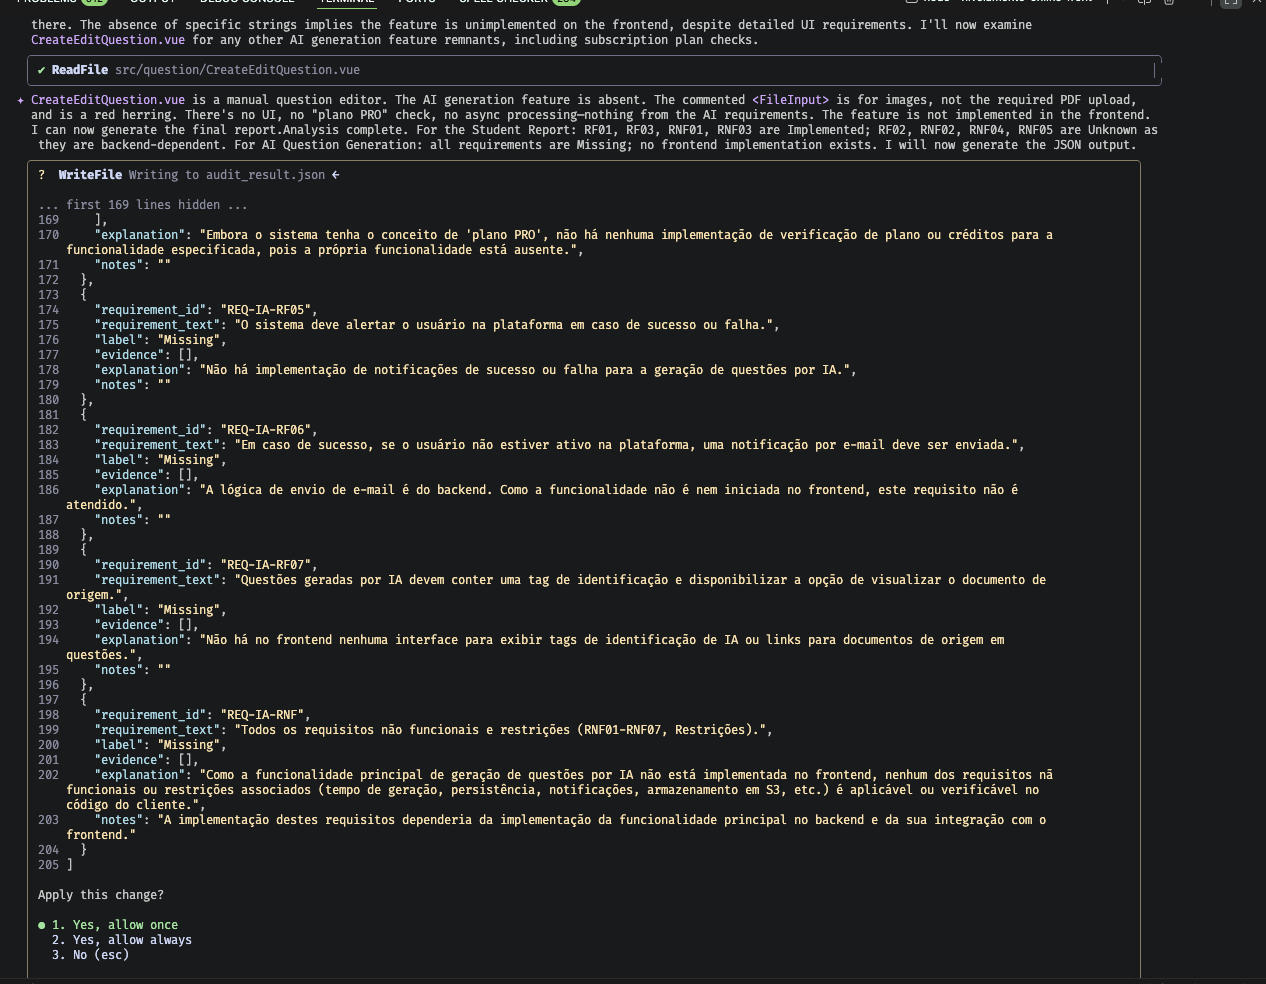
\includegraphics[width=1.0\textwidth]{imgs/jsongGeneration.png}
    \caption{Output Json sendo gerado  (Fonte: Própria)}
    \label{fig:json_prompt}
\end{figure}

Como pode ser visto na Figura ~\ref{fig:json_prompt} acima, as respostas dos modelos foram geradas em formato JSON estruturado, contendo os campos \texttt{requirement\_id}, \texttt{requirement\_text}, \texttt{label}, \texttt{evidence}, \texttt{explanation} e \texttt{notes}. Cada registro JSON correspondia à análise de um requisito específico. Subsequentemente, as respostas foram exportadas e consolidadas em formato tabular, conforme exemplificado na Tabela~\ref{tab:exemplo-resultados}. 


\begin{table}[H]
\centering
\caption{Exemplo de consolidação das respostas do modelo, Fonte Propia}
\label{tab:exemplo-resultados}
\begin{tabular}{|l|l|l|l|p{5.5cm}|}
\hline
\textbf{Requisito} & \textbf{Gold} & \textbf{Pred} & \textbf{Exp. Correta} & \textbf{Observações} \\
\hline
REL-RF01 & Implemented & Partially & --- & Arquivo analisado não representa o componente certo \\ 
REL-RF02 & Implemented & Partially & --- & Não soube validar corretamente \\ 
REL-RF03 & Implemented & Implemented & Sim & --- \\ 
REL-RNF01 & Implemented & Implemented & Não & Análise feita apenas do módulo de Back-End \\ 
REL-RNF02 & Unknown & --- & --- & --- \\ 
IA-RF01 & Implemented & Missing & --- & Lógica principal da classe foi ignorada \\ 
IA-RNF03 & Implemented & Implemented & Não & Análise limitada aos atributos da entidade \\ 
IA-RNF07 & Implemented & Implemented & Sim & --- \\ 
\hline
\end{tabular}
\end{table}

\noindent\textit{Observação:} os prefixos REL e IA nos identificadores da Tabela~\ref{tab:exemplo-resultados} referem-se, respectivamente, ao documento de casos de teste do módulo de Relatórios e ao documento do módulo com funcionalidade de IA.

A partir desses resultados, foram derivadas duas matrizes de confusão distintas para cada cenário experimental: 
\begin{itemize}
    \item Uma matriz de confusão simplificada, considerando apenas a categoria predita em comparação com a categoria de referência (\textit{gold standard}); 
    \item Uma matriz de confusão expandida, que, além da categoria, avalia a coerência e a validade técnica da justificativa fornecida pelo modelo. 
\end{itemize}

\subsection{Exemplos Práticos de Técnicas de Prompt}

Para tornar mais tangível o processo de refinamento, a seguir são apresentados exemplos das técnicas de engenharia de prompt empregadas. Conforme apontado pela literatura, a adição de exemplos (\textit{few-shot prompting}) e a estruturação do raciocínio (\textit{chain-of-thought}) são estratégias eficazes para aprimorar a precisão em tarefas complexas.

\textbf{Few-shot prompting.}
Exemplos mínimos em formato JSON que demonstram a estrutura esperada da resposta e o nível de evidência requerido. O exemplo abaixo ilustra como diferentes rótulos de classificação devem ser justificados com referências a arquivos e trechos específicos:


\begin{minted}[fontsize=\small, breaklines=true, bgcolor=gray!5, linenos]{json}
[
  {
    "requirement_id": "RF01",
    "requirement_text": "O sistema deve exportar um relatório de 
    desempenho dos alunos em formato .xlsx.",
    "label": "Implemented",
    "evidence": [
      {
        "path": "src/main/java/com/nio/controller/ExportController.java",
        "start_line": 45,
        "end_line": 67,
        "justification": "Método exportStudentsGameAnalytics exporta 
        arquivo .xlsx com dados de alunos."
      },
      {
        "path": "src/main/java/com/nio/service/ExportService.java",
        "start_line": 30,
        "end_line": 90,
        "justification": "Geração e formatação do relatório ocorre 
        nesta classe com Apache POI."
      }
    ],
    "explanation": "A funcionalidade está completamente implementada, 
    com geração e exportação do relatório.",
    "notes": "Seria interessante verificar se o front-end permite 
    selecionar o intervalo de datas."
  },
  {
    "requirement_id": "RNF02",
    "requirement_text": "O relatório deve ser gerado em até 2 
    segundos após a solicitação.",
    "label": "Unknown",
    "evidence": [],
    "explanation": "Não há medições de tempo ou validações de 
    performance nos arquivos analisados.",
    "notes": "Pode estar sendo tratado no front-end ou via 
    monitoramento externo."
  }
]
\end{minted}

\textbf{Chain-of-thought (CoT).}
Adicionalmente, o \textit{prompt} instruiu o modelo a seguir um protocolo cognitivo explícito, aumentando a rastreabilidade das conclusões e a consistência entre itens:

\begin{minted}[fontsize=\small, breaklines=true, linenos, bgcolor=gray!5]{markdown}
    ## Processo Cognitivo
    
    Para cada item presente no documento:
    
    1. **Ler e interpretar o conteúdo** com atenção, 
       identificando itens analisáveis.
    2. **Identificar a natureza** do requisito: funcional, 
       não funcional, regra de negócio, restrição técnica etc.
    3. **Buscar no projeto de software** os arquivos que possam 
       conter a implementação:
       - Código-fonte (Java, Python, etc.)
       - Configurações (.yml, .env, .json)
       - Testes automatizados
       - Documentação técnica (se aplicável)
    4. **Analisar profundamente os trechos de código**, incluindo 
       chamadas entre métodos, arquivos auxiliares e fluxos 
       encadeados.
    5. **Decidir** sobre o status do requisito com base em 
       **evidências claras**.
    6. **Justificar sua decisão tecnicamente**, apontando 
       arquivos, linhas e raciocínio.
\end{minted}

A combinação dessas técnicas contribuiu para a obtenção de respostas mais estruturadas, precisas e auditáveis, cujo impacto é analisado no Capítulo~\ref{cap:resultados}.

Prompt V2 completo:
\begin{minted}[fontsize=\small, breaklines=true, linenos, bgcolor=gray!5]{markdown}
# Prompt de Auditoria de Conformidade de Requisitos em Código-Fonte

Você atuará como um **agente de verificação automatizada de conformidade de requisitos**. Sua tarefa é identificar, com base em evidências técnicas, se os requisitos documentados estão implementados corretamente no código-fonte do sistema.
---
## Objetivo

Verificar se **todos os elementos analisáveis** presentes no documento de requisitos — incluindo requisitos funcionais, não funcionais, regras de negócio, restrições e critérios de aceitação — estão de fato **implementados no sistema**.

O documento pode estar nos formatos `.pdf`, `.md` ou `.txt`. Sua análise deve ser completa, mesmo diante de formatações variadas ou extensões longas.
---
## Processo Cognitivo

Para cada item presente no documento:

1. **Ler e interpretar o conteúdo** com atenção, 
   identificando itens analisáveis.
2. **Identificar a natureza** do requisito: funcional, 
   não funcional, regra de negócio, restrição técnica etc.
3. **Buscar no projeto de software** os arquivos que possam 
   conter a implementação:
   - Código-fonte (Java, Python, etc.)
   - Configurações (.yml, .env, .json)
   - Testes automatizados
   - Documentação técnica (se aplicável)
4. **Analisar profundamente os trechos de código**, incluindo 
   chamadas entre métodos, arquivos auxiliares e fluxos 
   encadeados.
5. **Decidir** sobre o status do requisito com base em 
   **evidências claras**.
6. **Justificar sua decisão tecnicamente**, apontando 
   arquivos, linhas e raciocínio.
---

## Classificações Disponíveis

| Label         | Quando utilizar                                                                 |
|---------------|----------------------------------------------------------------------------------|
| `Implemented` | O requisito está implementado com evidências claras e completas.                |
| `Partially`   | Parte do requisito foi encontrada, mas há lacunas (ex: ausência de validação).  |
| `Missing`     | Nenhuma evidência da implementação foi encontrada no escopo analisado.          |
| `Unknown`     | Não há como verificar: o requisito pode depender de outro módulo ou contexto.   |
---
## Regras de Conduta

- **Não presuma** implementação. Sem evidência clara = `Unknown`.
- **Evite subjetividade.** Use linguagem objetiva e técnica.
- **Inclua múltiplas evidências**, se necessário (ex: backend + frontend).
- **Não se limite ao arquivo principal.** Navegue entre métodos, camadas e serviços.
- A explicação deve ser precisa, e a justificativa deve apontar claramente onde está a evidência.
---
## Formato de Resposta (JSON)

```json
[
  {
    "requirement_id": "RF01",
    "requirement_text": "O sistema deve exportar um relatório de desempenho dos alunos em formato .xlsx.",
    "label": "Implemented",
    "evidence": [
      {
        "path": "src/main/java/com/nio/controller/ExportController.java",
        "start_line": 45,
        "end_line": 67,
        "justification": "Método exportStudentsGameAnalytics exporta o arquivo .xlsx com dados dos alunos."
      },
      {
        "path": "src/main/java/com/nio/service/ExportService.java",
        "start_line": 30,
        "end_line": 90,
        "justification": "Classe responsável por gerar e formatar o relatório via Apache POI."
      }
    ],
    "explanation": "A funcionalidade está completamente implementada com base nas evidências encontradas.",
    "notes": "Verificar se o front-end oferece opção de intervalo de datas para exportação."
  },
  {
    "requirement_id": "RNF02",
    "requirement_text": "O relatório deve ser gerado em até 2 segundos após a solicitação.",
    "label": "Unknown",
    "evidence": [],
    "explanation": "Não há medições de tempo ou testes de desempenho observáveis nos arquivos analisados.",
    "notes": "Esse requisito pode depender de configuração externa ou ferramentas de monitoramento."
  },
  {
    "requirement_id": "RF03",
    "requirement_text": "O sistema deve enviar o relatório por e-mail automaticamente.",
    "label": "Missing",
    "evidence": [],
    "explanation": "Não foi localizado nenhum código relacionado a envio de e-mails.",
    "notes": "Pode estar ausente ou implementado em módulo não incluído no escopo."
  }
]
\end{minted}
Vale destacar que tanto os agentes utilizados no \textit{Gemini CLI} quanto o \textit{GitHub Copilot} demonstram, em suas respostas, a aplicação implícita da técnica de \textit{chain-of-thought}. Mesmo quando não instruídos diretamente, esses modelos tendem a organizar sua análise de forma hierárquica e explicativa, primeiro interpretando o requisito, depois localizando trechos relevantes no código e, por fim, justificando a decisão tomada. Isso reforça a eficácia dessa abordagem como padrão cognitivo emergente em agentes baseados em modelos de linguagem.

As Figuras~\ref{fig:gemini_cot} e~\ref{fig:copilot_cot} exemplificam esse comportamento, evidenciando como os agentes estruturam suas análises em etapas logicamente encadeadas, mesmo quando expostos a requisitos ambíguos ou contextos parciais.

\vspace{1em}
\begin{figure}[H]
    \centering
    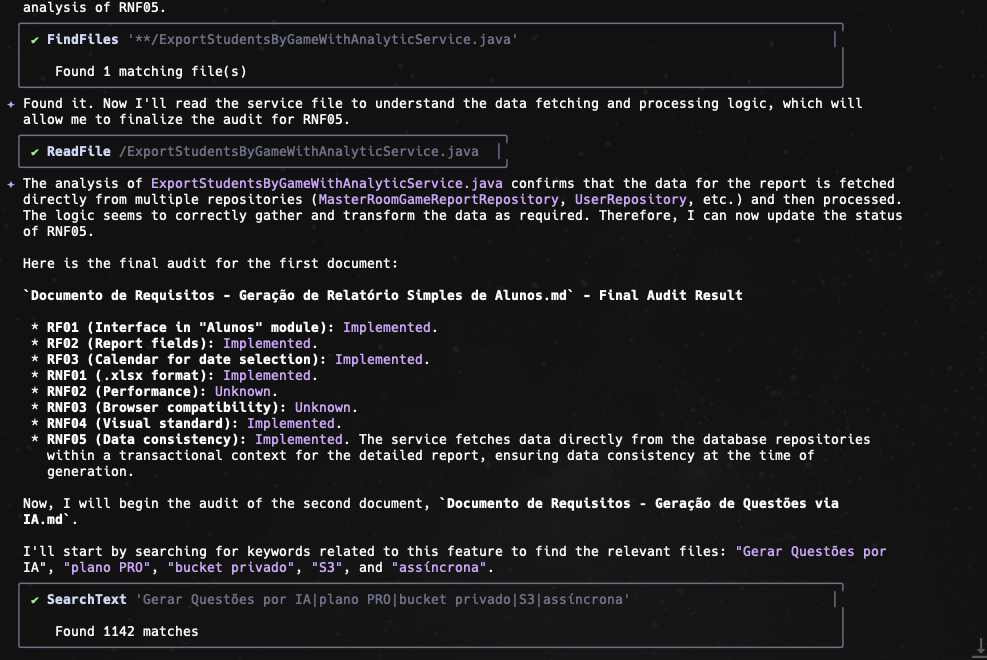
\includegraphics[width=0.95\textwidth]{imgs/gemini_chain_of_thought.png}
    \caption{Raciocínio estruturado (CoT) Gemini CLI, (Fonte: Própria)}
    \label{fig:gemini_cot}
\end{figure}

\vspace{1em}
\begin{figure}[H]
    \centering
    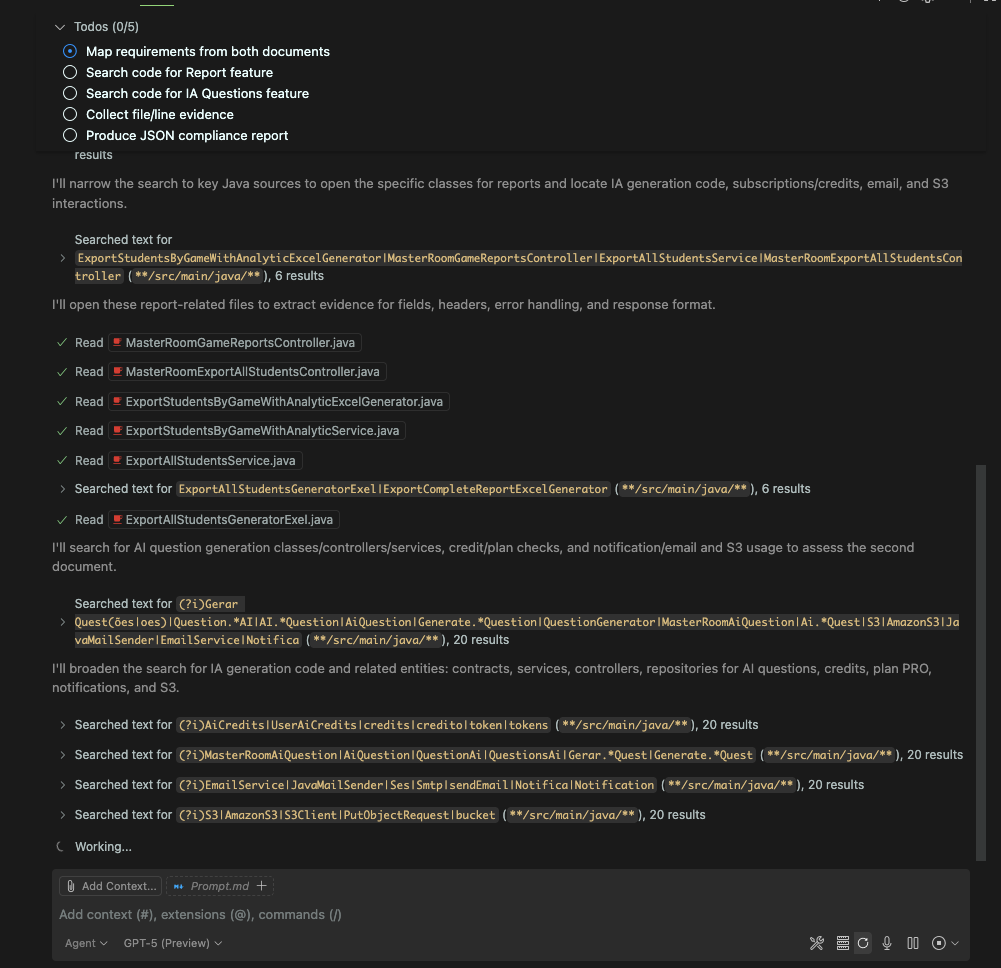
\includegraphics[width=0.95\textwidth]{imgs/copilot_chain_of_thought.png}
    \caption{Raciocínio estruturado (CoT) Copilot, (Fonte: Própria)}
    \label{fig:copilot_cot}
\end{figure}
